\documentclass[11pt,a4paper]{article}
\usepackage[top=3cm, bottom=2cm, left=2cm, right=2cm]{geometry}
\usepackage[utf8]{inputenc}
\usepackage{amsmath, amsfonts, amssymb}
\usepackage{siunitx}
\usepackage[brazil]{babel}
\usepackage{graphicx}
\usepackage[margin=10pt,font={small, it},labelfont=bf, textfont=it]{caption}
\usepackage[dvipsnames, svgnames]{xcolor}
\DeclareCaptionFont{MediumOrchid}{\color[svgnames]{MediumOrchid}}
\usepackage[pdftex]{hyperref}
\usepackage{natbib}
\bibliographystyle{plainnat}
\bibpunct{\textcolor{MediumOrchid}{\textbf{[}}}{\textcolor{MediumOrchid}{\textbf{]}}}{,}{s}{}{}
\usepackage{color}
\usepackage{footnote}
\usepackage{setspace}
\usepackage{booktabs}
\usepackage{multirow}
\usepackage{subfigure}
\usepackage{fancyhdr}
\usepackage{leading}
\usepackage{indentfirst}
\usepackage{wrapfig}
\usepackage{mdframed}
\usepackage{etoolbox}
\usepackage[version=4]{mhchem}
\usepackage{enumitem}
\usepackage{caption}
\usepackage{titlesec}
\usepackage{tcolorbox}
\usepackage{tikz}
\usepackage{LobsterTwo}
\usepackage[T1]{fontenc}
\usepackage{fontspec}
\usepackage{txfonts}
\usepackage[bottom]{footmisc}
\tcbuselibrary{skins,breakable}
\sisetup{output-decimal-marker={.}}

\makeatletter
\def\footnoterule{\kern-3pt\color{MediumOrchid}\hrule\@width0.6\textwidth height 0.8pt\kern2.6pt}
\makeatother

\renewcommand{\footnotelayout}{\itshape\color{MediumOrchid}}

\AtBeginEnvironment{equation}{\fontsize{13}{16}\selectfont}


\titleformat{\section}{\LobsterTwo\huge\color{CarnationPink}}{\thesection.}{1em}{}
\titleformat{\subsection}{\LobsterTwo\huge\color{CarnationPink}}{\thesubsection}{1em}{}
\titleformat{\subsubsection}{\bf\LobsterTwo\Large\color{MediumOrchid}}{\thesubsubsection}{1em}{}


\DeclareCaptionLabelFormat{figuras}{\textcolor{DarkTurquoise}{Figura \arabic{figure}}}
\captionsetup[figure]{labelformat=figuras}

\makeatletter
\renewcommand\tagform@[1]{\maketag@@@{\color{CarnationPink}(#1)}}
\makeatother

\renewcommand{\theequation}{Eq. \arabic{equation}}
\renewcommand{\thefigure}{Fig. \arabic{figure}}
\renewcommand{\thesection}{\textcolor{CarnationPink}{\arabic{section}}}

\setlist[itemize]{label=\textcolor{CarnationPink}{$\blacksquare$}}

\setlist[enumerate]{label=\textcolor{CarnationPink}{\arabic*.}, align=left, leftmargin=1.5cm}


\newcounter{exemplo}

\NewDocumentEnvironment{exemplo}{ O{} }{%
\allowbreak
\setlength{\parindent}{0pt}
  \begin{mdframed}[
  leftline=true,
  topline=false,
  rightline=false,
  bottomline=false,
  linewidth=2pt,
  linecolor=CarnationPink,
  frametitlerule=false,
  frametitlefont=\LobsterTwo\large\color{CarnationPink},
  frametitle={\color{CarnationPink}\LobsterTwo\large #1},
  ]
}{%
  \end{mdframed}
}

\setlength{\fboxsep}{5pt}
\setlength{\fboxrule}{1.5pt}
\usepackage{float}
\renewcommand{\thefootnote}{\alph{footnote}}
\usepackage{url}
\hypersetup{
	colorlinks=true,
	linkcolor=DarkTurquoise,
	filecolor=DarkTurquoise,      
	urlcolor=DarkTurquoise,
	citecolor=DarkTurquoise,
	pdftitle={Especialista em Física da Radioterapia}
}
\pagestyle{fancy}
\fancyhf{}
\renewcommand{\headrulewidth}{0pt}
\rfoot{\color{DarkTurquoise}\thepage \\ \LobsterTwo{\small\textcolor{CarnationPink}{@defDalila}}}


\title{\LobsterTwo\Huge{Controle de Qualidade}}
\author{\LobsterTwo\Large{QA e Comissionamento de Novas Tecnologias}\nocite{*}}
\date{\LobsterTwo\textit{Dalila Mendonça}}
\begin{document}
	\maketitle


\section{Introdução}

	Abrangentes testes de aceite e comissionamento de novos equipamentos são as bases para a implementação segura de novas tecnologias em um departamento de Radioterapia. Assim que a unidade estiver em pleno funcionamento, um programa de rotina de garantia de qualidade (QA) deve ser seguido para garantir que a unidade continue a funcionar dentro dos limites aceitáveis. Muitos dos testes de controle de qualidade dependerão de valores de baseline estabelecidos no momento do comissionamento. Além de verificar a funcionalidade e desempenho do equipamento, o pessoal que opera o equipamento deve ser devidamente treinado e avaliado quanto à competência para atuação na prática clínica. Políticas e procedimentos claros devem ser desenvolvidos antes da operação da instituição para garantir que todos os membros da equipe entendam o uso do equipamento e seu papel no processo clínico.

\section{Considerações Pré-Comissionamento e Aquisição do Equipamento}

	Antes da compra do equipamento, há considerações importantes a serem feitas para que a funcionalidade do acelerador atenda a necessidade clínica. É útil desenvolver uma \textcolor{MediumOrchid}{\textbf{\textit{solicitação de proposta (RFP)}}} detalhada contendo os recursos desejados para que vários sistemas possam ser comparados. A \ref{fig:aquisicaoLinac} mostra um exemplo para a compra de um linac. É importante observar a solicitação ao fornecedor de um \textcolor{MediumOrchid}{\textbf{\textit{documento de análise do modo de falha}}}. A disponibilidade de tal documento será útil na concepção de procedimentos e processos de controle de qualidade. Esta lista é um acréscimo à compilação padrão de especificações de parâmetros mecânicos e de feixe. A Comissão Eletrotécnica Internacional (IEC) descreveu as especificações de desempenho sugeridas. Se forem desejadas especificações diferentes dos valores do fabricante, elas devem ser descritas em um adendo de contrato antes da compra.

	\begin{figure}[!h]
		\centering

		\subfigure{
		\fcolorbox{DarkTurquoise}{white}{%
			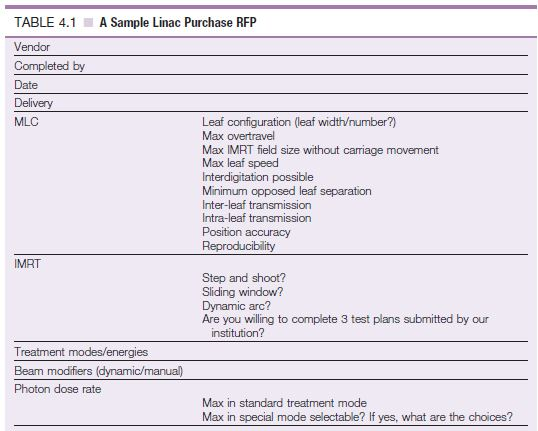
\includegraphics[width=0.5\textwidth]{Imagens/aquisicaoLinac1.JPG}
		}} \\ %
		\subfigure{
		\fcolorbox{DarkTurquoise}{white}{%
			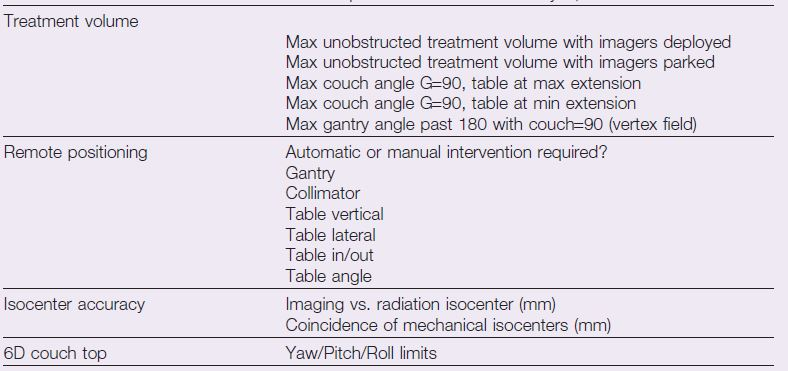
\includegraphics[width=0.5\textwidth]{Imagens/aquisicaoLinac2.JPG}
		}} \\%
		\subfigure{
		\fcolorbox{DarkTurquoise}{white}{%
			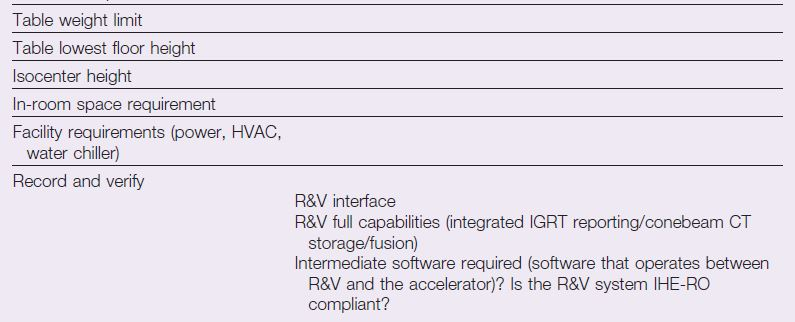
\includegraphics[width=0.5\textwidth]{Imagens/aquisicaoLinac3.JPG}
		}} \\%
		\subfigure{
		\fcolorbox{DarkTurquoise}{white}{%
			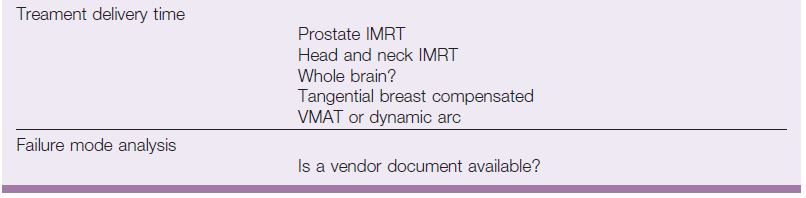
\includegraphics[width=0.5\textwidth]{Imagens/aquisicaoLinac4.JPG}
		}} \\%
		\caption{Aquisição Linac}
		\label{fig:aquisicaoLinac}
	\end{figure}

	O fabricante deve identificar se cada \textcolor{MediumOrchid}{\textbf{\textit{recurso do sistema}}} desejado está disponível no momento ou se é um trabalho em andamento. Além dos recursos do sistema, o \textcolor{MediumOrchid}{\textbf{\textit{procedimento de aceite}}} do fornecedor deve ser examinado para garantir que as especificações do fornecedor correspondam às expectativas.

	O objetivo de uma rigorosa investigação de pré-venda é obter o sistema que melhor atenda às necessidades da clínica com o melhor custo. Cada clínica é diferente e terá prioridades diferentes, portanto, um método deve ser estabelecido para pesar os diferentes fatores de acordo com as necessidades locais. Por exemplo, ao selecionar um linac, os recursos a serem considerados incluem \textcolor{MediumOrchid}{\textbf{\textit{velocidade de entrega, precisão de entrega, conformidade de entrega, resolução de imagem, modalidades de imagem, gerenciamento de movimento, facilidade de uso, integração com sistemas existentes, confiabilidade, serviço e marketing}}}. Para obter uma comparação de custo confiável, é recomendável incluir pelo menos 5 anos de custo de serviço.

	Muitas \textcolor{MediumOrchid}{\textbf{\textit{questões logísticas}}} também devem ser resolvidas ou esclarecidas antes da compra. Por exemplo, qual é o caminho de entrega pelo hospital? O equipamento caberá em todos os corredores e aberturas de portas? A entrega após o expediente ou no fim de semana será necessária e terá um custo extra? A equipe de instalação exigirá autorização do hospital para estar no local? Serão necessárias modificações na blindagem? Quais são as contingências se houver um atraso na construção? Após a conclusão da compra, devem ser realizadas reuniões regulares com o gerente de projeto do fornecedor, a equipe de construção e a equipe de radioterapia para garantir uma instalação tranquila assim como os testes de aceite.

\section{Comissionamento e Testes de Aceite}

\subsection*{Aceleradores Lineares}

	Existem muitos documentos que descrevem o comissionamento e o controle de qualidade de aceleradores lineares utilizados em radioterapia. Os testes de comissionamento podem ser separados em sete categorias:

	\begin{enumerate}
		\item \textcolor{DarkTurquoise}{\textbf{\textit{Adequação da Blindagem}}}. Um monitoramento preliminar deve ser feito imediatamente após o linac ser capaz de fazer um feixe para garantir a segurança do pessoal que realiza o teste e o pessoal das áreas vizinhas. Um monitoramento completo da blindagem e da fuga do cabeçote pode ser feito posteriormente.
		\item \textcolor{DarkTurquoise}{\textbf{\textit{Teste de intertravamentos de segurança}}};
		\item \textcolor{DarkTurquoise}{\textbf{\textit{Teste de parâmetros mecânicos}}}, como gantry, colimador, MLC e mesa. Cada um é testado para funcionalidade e desempenho dentro da especificação.
		\item \textcolor{DarkTurquoise}{\textbf{\textit{Medidas de parâmetros do feixe}}}, como energia, planura, simetria, penumbra, transmissão dos jaws colimadores, transmissão da lâmina do MLC, transmissão inter-lâminas, transmissão do filtro, linearidade das unidades monitoras (MU), estabilidade de feixe versus ângulo de gantry, fatores de output, fatores de cone e  distância virtual da fonte;
		\item \textcolor{DarkTurquoise}{\textbf{\textit{Teste dos componentes de imagem}}};
		\item \textcolor{DarkTurquoise}{\textbf{\textit{Medida da precisão de entrega do plano do paciente}}}.
		\item \textcolor{DarkTurquoise}{\textbf{\textit{Auditoria externa por uma agência}}} como o Imaging and Radiation Oncology Core (IROC Houston) (anteriormente Radiological Physics Center (RPC)). Isso inclui verificações da saída da máquina e também a irradiação dos phantoms de teste. Isto ainda não é bem estabelecido no Brasil mas existem discussões entre a ABFM e e CNEN nesta direção.
	\end{enumerate}

\subsubsection*{Interlocks de Segurança}

	O teste dos intertravamentos de segurança pode variar de um simples teste do interlock da porta, abrindo a porta, a um teste complexo do interlock de simetria, direcionando o feixe até que o interlock acione e então medindo a simetria. Os testes mais complexos podem não ser necessários se for realizada uma análise de risco mostrando que a probabilidade de falha é baixa.

\subsubsection*{Testes Mecânicos}

	O teste dos parâmetros mecânicos é bastante direto e bem descrito nos documentos do fornecedor. A sequência do teste, no entanto, é muito importante, pois os ajustes de um parâmetro podem afetar outro. Um exemplo de sequência de execução dos testes pode ser o seguinte:

	\begin{enumerate}[label=\textcolor{CarnationPink}{\arabic*${}^\circ $}]
		\item \textcolor{DarkTurquoise}{\textbf{Defina o nível do gantry para o correto ângulo do gantry de \ang{0}.}} Este deve ser o primeiro passo pois todas as outras verificações irão depender do gantry. Depois que o zero verdadeiro for estabelecido, identifique a superfície na face do colimador onde um nível bolha pode ser colocado para confirmar o zero com segurança. Um nível de alta qualidade com indicadores de 0 e 90 graus é uma ferramenta necessária para um físico médico. Níveis digitais podem ser utilizados, mas a precisão deve ser validada. A precisão de qualquer nível pode ser verificada colocando-o em uma superfície nivelada e girando o nível 180 graus para confirmar a leitura.
		
		\item \textcolor{DarkTurquoise}{\textbf{Confirme a precisão do ângulo do gantry em outros ângulos.}} Use a superfície previamente identificada na face do colimador e o nível bolha para verificar os ângulos de \ang{90}, \ang{180} e \ang{270}.
		
		\item \textcolor{DarkTurquoise}{\textbf{Confirme a coincidência do campo radiativo campo luminoso.}} Verifique marcando o campo luminoso no filme e depois expondo o filme. Execute para tamanhos de campo pequenos, médios e grandes para todas as energias de fótons. Garantir uma tolerância muito rígida ($<$1 mm) nesta etapa permitirá o uso do campo luminoso em algumas verificações citadas abaixo. Existem placas disponíveis comercialmente com marcações radiopacas das bordas do campo, incorporadas à placa que eliminam a necessidade de marcação manual do campo luminoso (Como os isoalign da Sun Nuclear e Civco). Alguns destes dispositivos podem ser utilizados com EPID em vez de filme.
		
		\item \textcolor{DarkTurquoise}{\textbf{Confirme a concentricidade dos jaws e a precisão da sua posição.}} Verifique marcando o campo luminoso em um papel milimetrado e girando o colimador 180 graus para confirmar se o campo luminoso ainda coincide com as marcas realizadas.
		
		\item \textcolor{DarkTurquoise}{\textbf{Confirme a centralização do retículo.}} Isso pode ser verificado junto com a Etapa 3, marcando o centro do retículo. Verifique também se o centro do retículo se projeta ao longo de uma linha vertical verdadeira. Isso pode ser feito transferindo onde o retículo se projeta no isocentro para o chão usando um prumo\footnote{instrumento constituído de corpo pesado com uma alça na base, amarrado a um fio flexível, para verificar a verticalidade de um lugar ou o eixo.} e, em seguida, confirmando que a projeção do retículo corresponde à projeção do prumo.
	
		\item \textcolor{DarkTurquoise}{\textbf{Confirme o isocentro mecânico.}} Isso geralmente é feito usando uma ponteira mecânica frontal. Coloque uma ponteira na mesa de tratamento estendendo-se para fora da borda superior. No ângulo do gantry \ang{0}, defina a ponteira mecânica para 100 cm. Alinhe a ponteiro na mesa com a ponteira frontal. Gire o gantry em toda a sua faixa de movimento e confirme se o desvio máximo está dentro das especificações. Isso também confirma a precisão da ponteira frontal. Se houver um deslocamento consistente, a ponteira frontal precisa ser ajustada. Neste ponto, alinhe os lasers ao isocentro mecânico do gantry.
		
		\item \textcolor{DarkTurquoise}{\textbf{Confirme a coincidência do isocentro mecânico com o isocentro radiativo.}} Verifique com filme usando a técnica tradicional de irradiação em estrela (star shot). Marque a localização do isocentro mecânico no filme antes de expo-lo. Ao avaliar o filme, há dois parâmetros a serem medidos: Primeiro, verifique se a interseção dos feixes de vários ângulos do gantry está dentro da especificação; Em segundo lugar, verifique se o isocentro mecânico coincide com o isocentro radiativo.
		
		\item \textcolor{DarkTurquoise}{\textbf{Defina os lasers para o isocentro radiativo.}} Deve-se ter cuidado para garantir que os lasers estejam nivelados e ortogonais e que os lasers opostos se coincidam. O uso de um prumo pode ajudar na verificação do nível. Outra ferramenta que pode ajudar na configuração do laser é um laser utilizado em construção autonivelante de três direções (three-direction, self-leveling laser). Ele pode ser colocado no isocentro e utilizado para projetar linhas de nível dos lases nas paredes, no chão e no teto. O dispositivo deve ser verificado quanto à calibração adequada antes de usar.
		
		\item \textcolor{DarkTurquoise}{\textbf{Confirme o isocentro do colimador.}} Isso também é medido com um filme usando uma técnica de irradiação em estrela. Marque o centro do retículo no filme antes de expor. Verifique a coincidência dos feixes e a concordância do centro com o retículo.
		
		\item \textcolor{DarkTurquoise}{\textbf{Confirme a precisão do ângulo do colimador.}} Com o gantry em \ang{0}, defina um dos jaws na posição 0 (centro do campo) na direção do plano. Abra os demais jaws completamente. Fixe um pedaço de papel milimetrado no tampo da mesa e marque o centro do feixe. Gire o Gantry em ambas as direções de modo que seja possível ver a projeção da luz de campo no papel. A borda do jaw deverá permanecer na marca central durante todo o movimento do gantry se o jaw estiver exatamente paralelo ao movimento do gantry, indicando um ângulo zero verdadeiro do colimador. Ângulos de colimador de \ang{90}, \ang{180} e \ang{270} podem ser testados de forma semelhante. Ângulos intermediários podem ser testados alinhando um transferidor ao centro e observando o ângulo indicado pelo retículo.
		
		\item \textcolor{DarkTurquoise}{\textbf{Confirme a precisão da posição do colimador.}} Varie a configuração do jaw/lâmina do colimador e observe o campo luminoso em comparação com uma régua calibrada ou papel milimetrado. A precisão da posição do MLC também pode ser verificada com EPID ou filme.
		
		\item \textcolor{DarkTurquoise}{\textbf{Confirme se o movimento vertical da mesa está paralelo ao feixe.}} Cole um pedaço de papel no tampo da mesa e marque o centro do feixe. Defina o ângulo do gantry para \ang{0} usando um nível para garantir a precisão da análise. Abaixe e levante a mesa enquanto observa o campo luminoso. Se a mesa estiver se deslocando em um caminho vertical verdadeiro, o retículo permanecerá na marca central.
		
		\item \textcolor{DarkTurquoise}{\textbf{Confirme a precisão da posição vertical da mesa.}} Levante a parte superior da mesa de modo que os lasers apenas toquem a parte superior da mesa. Confirme se a leitura vertical da mesa é 0. Fixe uma régua calibrada na lateral da mesa na direção vertical. Confirme se a leitura vertical da mesa durante o movimento vertical corresponde à régua observando onde o laser atinge a régua.
		
		\item \textcolor{DarkTurquoise}{\textbf{Confirme o isocentro radiativo da mesa.}} Isso é medido com filme usando uma técnica de star shot. Marque o centro do retículo no filme antes de irradiar o feixe. Verifique a coincidência dos feixes e a concordância do centro com o retículo.
		
		\item \textcolor{DarkTurquoise}{\textbf{Confirme se a mesa se desloca em linha reta ao ser deslocada longitudinalmente em direção ao gantry.}} Cole um pedaço de papel na parte superior da mesa e marque o centro do feixe. Desloque a mesa para dentro e para fora enquanto observa o campo luminoso. Se a mesa estiver se movendo em linha reta, o retículo permanecerá alinhado à marca durante todo o curso.
		
		\item \textcolor{DarkTurquoise}{\textbf{Confirme a precisão do ângulo da mesa.}} Confirme o ângulo \ang{0} da mesa usando o teste na Etapa 15. Os ângulos da mesa de \ang{90} e \ang{270} podem ser testados de forma semelhante. Ângulos intermediários podem ser testados alinhando um transferidor ao centro e observando o ângulo indicado pelo retículo.
		
		\item \textcolor{DarkTurquoise}{\textbf{Confirme a precisão do deslocamento da mesa.}} Coloque uma régua calibrada no tampo da mesa e mova a mesa por distâncias conhecidas observando o retículo. Verifique ambas as direções de deslocamento em toda a amplitude de movimento. Um peso uniformemente distribuído deve ser adicionado ao tampo da mesa para simular condições clínicas. Isso pode ser feito com água sólida ou phantoms antropomórficos.
		
		\item \textcolor{DarkTurquoise}{\textbf{Confirme a inclinação da mesa para várias extensões.}} Cole uma régua na lateral da mesa na direção vertical. Alinhe o laser para uma posição conveniente de, por exemplo, 10 cm na régua. Adicione peso à mesa conforme descrito na Etapa 17 e observe a mudança no local onde o laser atinge a régua.
		
		\item \textcolor{DarkTurquoise}{\textbf{Confirme a precisão do indicador óptico de distância (ODI).}} Coloque placas de espessura precisa em cima do tampo da mesa. Ajuste a mesa verticalmente até que os lasers toquem o topo das placas. Confirme se esta é uma distância fonte-superfície (SSD) de 100 cm usando a ponteira mecânica frontal. Confirme se o ODI lê 100 cm dentro das especificações. Remova as placas uma a uma e confirme se a SSD indica 100 $+$ a espessura total da placa removida para cada uma das placas utilizadas. Para verificar a SSD $<$ 100 cm, ajuste a posição vertical da mesa para que a parte superior da mesa fique a 100 cm e, em seguida, adicione as placas uma de cada vez enquanto verifica a SSD em cada etapa.

	\end{enumerate}

	Todo esse processo pode facilmente levar um dia inteiro, principalmente se for necessário fazer ajustes. O processo de comissionamento é o momento de tornar todos os parâmetros o mais precisos possível. \textcolor{MediumOrchid}{\textbf{\textit{Existem incertezas nas medidas e o desempenho do equipamento provavelmente diminuirá no futuro}}}. Por esses motivos, os parâmetros devem ser ajustados para ficarem dentro da especificação, de modo que ajustes não sejam necessários em um futuro próximo. Isso pode exigir alguma negociação diplomática com o engenheiro de instalação para continuar ajustando um parâmetro, mesmo que esteja dentro das especificações. Existem dispositivos comerciais disponíveis que podem tornar alguns desses testes mais eficientes.

\subsubsection*{Parâmetros do Feixe}

	A medida dos parâmetros do feixe deve ser realizada com a maior precisão porque o comissionamento inicial será utilizado para modelagem de dados do feixe e formará a base de comparação para todas as medidas futuras de controle de qualidade. AAPM TG-106, \textit{``Accelerator Beam Data Comissioning Equipment and Procedures''}, inclui uma excelente descrição de como comissionar feixes de fótons e elétrons.

	Assim como no teste mecânico, a ordem da coleta de dados do feixe é importante. Um exemplo de sequência pode ser o seguinte:

	\begin{enumerate}[label=\textcolor{CarnationPink}{\arabic*${}^\circ $}]
		\item \textcolor{DarkTurquoise}{\textbf{Confirme se o feixe está perpendicular ao nível e centralizado no eixo de rotação do colimador.}} Depois de nivelar cuidadosamente o tanque de água e os mecanismos de movimentação do detector, execute os perfis no plano inline e no plano crossline em duas profundidades, uma em profundidade rasa ($d_{max}$) e outra em profundidade maior (20 ou 30 cm). Os centros das varreduras devem coincidir. Este processo de localização do eixo central (CAX) pode ser automatizado com alguns sistemas de escaneamento de tanques de água. Observe que o movimento do detector é confirmado para ser vertical usando os retículos que foram verificados na Etapa 5 acima. Para verificar a centralização do feixe no eixo do colimador, execute varreduras nos ângulos do colimador de \ang{0} e \ang{180} e confirme se as varreduras correspondem. 
		
		\item \textcolor{DarkTurquoise}{\textbf{Confirme a energia do feixe.}} Realize varreduras de dose de profundidade e confirme se o parâmetro relevante para determinar a energia do feixe está está dentro da especificação (ou seja, a porcentagem de dose na profundidade de 10 cm para fótons e profundidade das isodose de  (90\%) ou 50\%  para elétrons). Isso deve ser verificado antes dos demais testes porque alterações resultantes da corrente do ímã de dobra ou na potência de radiofrequência (RF) podem afetar as etapas subsequentes.
		
		\item \textcolor{DarkTurquoise}{\textbf{Confirme a simetria e a planura do feixe.}} Meça perfis para grandes campos em $d_{max}$ e a 10 cm de profundidade para confirmar a simetria e a planura do feixe. A simetria deve ser $<$ 1\% e a planura deve estar dentro das especificações do fornecedor. Se o direcionamento do feixe for necessário, repita a Etapa 1. Existem diferentes definições para a planura; certifique-se de que o planura seja medida de maneira consistente.
		
		\item \textcolor{DarkTurquoise}{\textbf{Verifique a estabilidade da viga em relação ao ângulo do gantry.}} Isso pode ser feito facilmente com uma matriz de detectores conectada a um suporte de gantry especial.
		
		\item Uma vez confirmados, os dados de dose em profundidade, perfil, fator de transmissão e dependência do tamanho do campo podem ser coletados. Após, os dados no ar podem então ser coletados. A medida da dose absoluta deve ser feita por último porque os ajustes nos outros parâmetros podem afetar a produção.
	
	\end{enumerate}

	Ao coletar dados de feixe, deve-se tomar cuidado na escolha dos detectores. Existem inúmeras considerações, a maioria das quais são discutidas no AAPM TG-106. Por exemplo, \textcolor{MediumOrchid}{\textbf{\textit{grandes câmaras de ionização não determinarão com precisão a penumbra do feixe}}}. Os \textcolor{MediumOrchid}{\textbf{\textit{diodos podem responder em excesso fora do campo}}}. Para \textcolor{MediumOrchid}{\textbf{\textit{feixes de elétrons}}}, \textcolor{MediumOrchid}{\textbf{\textit{se uma câmara de ionização for usada, as PDPs devem ser deslocadas e convertidas com razão do poder de freamento}}} dependentes da profundidade. Este não é o caso se um diodo for utilizado, embora seja necessário tomar cuidado ao escolher \textcolor{MediumOrchid}{\textbf{\textit{diodos de elétrons}}} versus fótons para a varredura (a diferença está na blindagem para fótons espalhados de baixa energia).

\subsubsection*{QA Contínuo}

	Após a conclusão do comissionamento, o escopo do controle de qualidade ao longo da rotina deve ser estabelecido de acordo com os documentos de referência, em particular o \textcolor{MediumOrchid}{\textbf{\textit{TG-142}}} sobre controle de qualidade de aceleradores lineares médicos e outros relatórios. \textcolor{MediumOrchid}{\textbf{\textit{As medidas do baseline do controle de qualidade diário, mensal e anual devem ser feitas no momento do comissionamento}}} para estabelecer um baseline adequado. \textcolor{MediumOrchid}{\textbf{\textit{No momento de cada controle de qualidade anual, as medidas diárias e mensais do controle de qualidade também devem ser realizadas}}} para garantir a fidelidade contínua dessas medidas. A descrição do teste, equipamento utilizado, frequência, quem realiza o teste, faixas aceitáveis e ações corretivas a serem tomadas devem ser documentadas para cada teste.

\subsubsection*{QA após Reparo}

	Outra situação que requer controle de qualidade é após um reparo significativo do equipamento. \textcolor{MediumOrchid}{\textbf{\textit{A instalação deve estabelecer um protocolo para quais medidas devem ser feitas após diferentes tipos de reparos}}}. Os fornecedores podem fornecer documentos de orientação, mas cada instalação deve estabelecer sua própria política. Um exemplo é mostrado na \ref{fig:qaAposReparo}.

	\begin{figure}[!h]
		\centering
		\fcolorbox{DarkTurquoise}{white}{%
			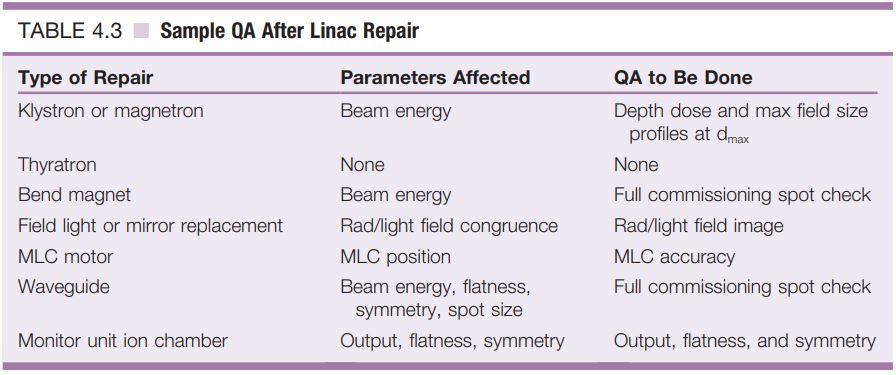
\includegraphics[width=0.8\textwidth]{Imagens/qaAposReparo.JPG}
		}%
		\caption{Exemplos de parâmetros afetados após determinados reparos}
		\label{fig:qaAposReparo}
	\end{figure}

	\textcolor{MediumOrchid}{\textbf{\textit{Documentar os problemas da máquina e sua forma de resolver}}} é uma importante atividade de controle de qualidade. A instalação deve ter um registro dos problemas da máquina, como eles foram resolvidos, qual controle de qualidade foi feito para e autorização para retorno ao serviço pelo físico médico. O tempo de inatividade (down time) deve ser documentado mensalmente e as tendências de reparo analisadas para quaisquer problemas contínuos. Um registro deve incluir no mínimo a data, hora, terapeuta presente, quem foi notificado (biomédico, físico, gerente, serviço), ações tomadas para resolver o problema, chamado de serviço feito se não for possível resolver, tempo de inatividade, tempo de atraso, número de pacientes não atendidos, horário de atendimento, acompanhamento e autorização física de retorno ao uso para cada incidente.

\subsection*{Unidades de Afterloading de Alta Taxa de Dose}

	Os sistemas de \textcolor{MediumOrchid}{\textbf{\textit{afterloader remoto}}} de alta taxa de dose (HDR) têm sido de uso comum desde a década de 1990. Normalmente, eles usam uma \textcolor{MediumOrchid}{\textbf{\textit{única fonte de \ce{^{192}Ir}}}} montada na \textcolor{MediumOrchid}{\textbf{\textit{extremidade de um longo fio}}} que é controlado por computador para conduzir a fonte até a distância apropriada e, em seguida, passar por uma série de \textcolor{MediumOrchid}{\textbf{\textit{posições de parada}}} para administrar a dose prescrita. As unidades possuem de \textcolor{MediumOrchid}{\textbf{\textit{5 a 20 canais}}}, permitindo tratamentos com múltiplos cateteres ou aplicadores. Os fornecedores incluem Elekta (anteriormente Nucletron) e Varian. Uma unidade mais nova, BEBIG Multisource, tem várias fontes, uma \ce{^{192}Ir} e \ce{^{60}Co}.

	Os \textcolor{MediumOrchid}{\textbf{\textit{testes de aceite e comissionamento}}} para afterloaders HDR são descritos \textcolor{MediumOrchid}{\textbf{\textit{TG-41}}} e envolvem a conclusão de todos os testes listados na \ref{fig:hdrguidelines}, bem como o comissionamento do sistema de planejamento de tratamento (TPS). Muitos dos testes envolvem o uso de filme para produzir auto-radiografias. Recentemente, foram descritos métodos usando imagens de portal e arrays de câmaras para realizar alguns dos testes de controle de qualidade. 


	\begin{figure}[!h]
		\centering
		\fcolorbox{DarkTurquoise}{white}{%
			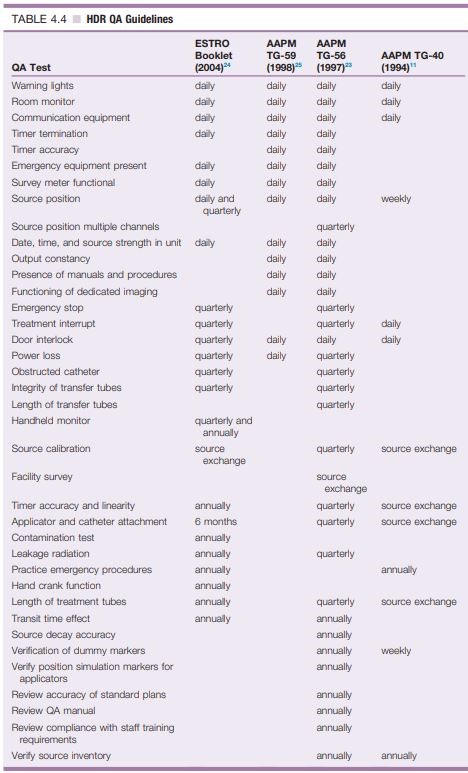
\includegraphics[width=0.6\textwidth]{Imagens/hdrguidelines.JPG}
		}%
		\caption{Guidelines para os QA de HDR}
		\label{fig:hdrguidelines}
	\end{figure}

	Há alguma discrepância entre as diretrizes sobre quais testes devem ser realizados e a frequência dos testes. Sem um documento de referência descrevendo a eficácia relativa de cada teste de controle de qualidade, modos de falha e análise de risco, seria prudente adotar a a maior frequência de teste.

	Além desses testes, o  TG-56 \textit{``Code of Practice for Brachytherapy Physics''} e o ESTRO24 recomendam um \textcolor{MediumOrchid}{\textbf{\textit{método terciário para verificação da intensidade da fonte}}}. Isso geralmente é feito com uma câmara de ionização cilíndrica em uma geometria fixa. Um \textcolor{MediumOrchid}{\textbf{\textit{valor de constância}}} pode ser estabelecido no comissionamento inicial do sistema. É importante reproduzir o setup com precisão, incluindo a proximidade de qualquer material espalhador (mesa de tratamento, paredes, pisos, etc.) para obter resultados consistentes. \textcolor{MediumOrchid}{\textbf{\textit{É útil ter este sistema de verificação de calibração de backup em caso de mau funcionamento da câmara  poço}}} (que é o dispositivo recomendado para medir a atividade da fonte) ou para \textcolor{MediumOrchid}{\textbf{\textit{solucionar problemas entre o certificado de calibração e a atividade medida localmente}}}. Outra boa prática é \textcolor{MediumOrchid}{\textbf{\textit{calibrar tanto a fonte antiga quanto a nova no momento da troca da fonte}}}. Isso fornece uma \textcolor{MediumOrchid}{\textbf{\textit{verificação da constância da câmara do poço}}}.

\subsection*{Unidades de Quilovoltagem}

	Unidades de tratamento com energias na faixa de quilovoltagem podem variar de equipamentos de \textcolor{MediumOrchid}{\textbf{\textit{raios-x superficial}}} até \textcolor{MediumOrchid}{\textbf{\textit{braquiterapia eletrônica}}} e \textcolor{MediumOrchid}{\textbf{\textit{ortovoltagem}}}. As unidades de \textcolor{MediumOrchid}{\textbf{\textit{raios-x superficiais e de ortovoltagem}}} normalmente realizam tratamentos usando \textcolor{MediumOrchid}{\textbf{\textit{aplicadores fixos com SSDs relativamente pequenas}}}. Elas também usam combinações de \textcolor{MediumOrchid}{\textbf{\textit{filtros adicionais}}} para obter diferentes qualidades de penetração. As unidades de \textcolor{MediumOrchid}{\textbf{\textit{braquiterapia eletrônica}}} são usadas nos tratamentos \textcolor{MediumOrchid}{\textbf{\textit{intraoperatórios}}} ou para tratar \textcolor{MediumOrchid}{\textbf{\textit{lesões cutâneas superficiais}}}. A braquiterapia eletrônica consiste no uso de uma \textcolor{MediumOrchid}{\textbf{\textit{fonte kV de baixa energia}}} (normalmente 50 kV) para fornecer radiação dentro ou adjacente a um tumor, semelhante aos métodos de braquiterapia que usam sementes radioativas. Porém, ao invés de uma semente radioativa, o \textcolor{MediumOrchid}{\textbf{\textit{alvo do dispositivo kV é colocado no local desejado}}}. O \textcolor{MediumOrchid}{\textbf{\textit{TG-152}}}, a resposta da AAPM de 2007 à solicitação de recomendações do CRCPD para os regulamentos modelo do CRCPD para braquiterapia eletrônica, contém seções relacionadas à calibração e controle de qualidade para essas unidades. O Comitê de Tecnologia Emergente da ASTRO também publicou um relatório em 2010 que analisa essas tecnologias.

	As unidades de braquiterapia eletrônica apresentam desafios especiais devido às curtas distâncias envolvidas, como mencionado anteriormente. Além disso, a instalação pode não ter uma câmara à prova d'água apropriada para medir o output ou a dose na profundidade. Devido à baixa energia, \textcolor{MediumOrchid}{\textbf{\textit{as câmaras de placas paralelas}}} são as preferidas. Estas são mais difíceis de serem a prova d'agua e podem ser necessários revestimentos finos. Deve-se tomar cuidado para selecionar um detector apropriado e aplicar as correções apropriadas. Parece haver consenso de que \textcolor{MediumOrchid}{\textbf{\textit{as câmaras de placas paralelas NACP, Markus, Advanced Markus e Roos podem ser usadas para medir a dose de profundidade com 3\% de incerteza}}}. A aplicação de fatores de correção dependentes da profundidade pode reduzir essa incerteza. \textcolor{MediumOrchid}{\textbf{\textit{Câmaras cilíndricas podem ser usadas, mas não podem medir com precisão nas regiões próximas da superfície}}} porque parte da câmara está acima da superfície da água nessa faixa. Nas profundidades além de 4 a 5 mm estas câmaras podem produzir resultados precisos.

\section{Unidades de Imagem}

\subsection*{Tomografia Computadorizada}

	O controle de qualidade das unidades de simulação de tomografia computadorizada (CT) é descrito no AAPM TG-66. Dependendo dos regulamentos estaduais, a unidade pode ter que cumprir alguns ou todos os requisitos de TC de diagnóstico. As descrições de teste no \textcolor{MediumOrchid}{\textbf{\textit{AAPM TG-66}}} são bem definidas e não precisam de elaboração. Um resumo dos testes recomendados é mostrado na \ref{fig:qaCtSimulador}.

	\begin{figure}[!h]
		\centering
		\fcolorbox{DarkTurquoise}{white}{%
			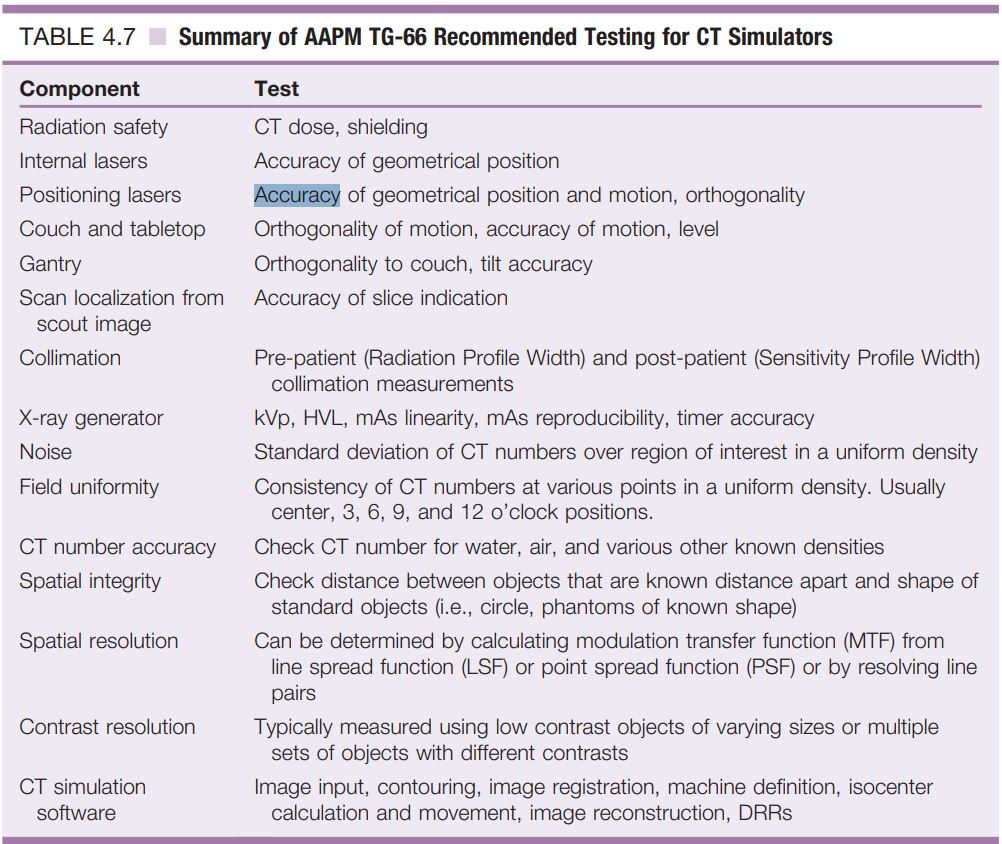
\includegraphics[width=0.7\textwidth]{Imagens/qaCtSimulador.JPG}
		}%
		\caption{Testes Recomendados Pra CT simulador}
		\label{fig:qaCtSimulador}
	\end{figure}

	Uma questão mencionada na AAPM TG-66 que merece consideração especial é a remoção e substituição do tampo plano da mesa. Se for uma unidade dedicada à Radioterapia, o tampo plano provavelmente permanecerá no lugar. Isso pode causar um problema com o posicionamento do phantom de QA, pois alguns phantoms são projetados para serem montados usando o mesmo mecanismo de encaixe usado pelo tampo plano. Portanto, uma nova montagem personalizada pode precisar ser projetada. Alternativamente, o phantom pode ser colocado no topo do encaixe ao invés de ser suspenso na extremidade da mesa. Deve-se observar que a presença do tampo da mesa alterará alguns dos valores do teste e será necessário estabelecer baselines diferentes dos valores especificados pelo fabricante. Se a unidade for compartilhada com radiologia diagnóstica, a remoção e substituição podem ser frequentes e o alinhamento adequado deve ser verificado diariamente. Estão disponíveis dispositivos comerciais que tornam os testes recomendados pela AAPM TG-66 mais eficientes. O Quasar Beam Geometry Phantom (Modus Medical) e CT Sim Check (Integrated Medical Technologies) são exemplos.

\subsection*{Unidades de Ultrassom}

	O uso do ultrassom (US) em Radioterapia é empregado principalmente para o \textcolor{MediumOrchid}{\textbf{\textit{tratamento do câncer de próstata}}}, seja em feixe externo ou braquiterapia intersticial. Além disso, a US pode ser utilizada para \textcolor{MediumOrchid}{\textbf{\textit{localização de tratamentos de boost de mama}}} ou \textcolor{MediumOrchid}{\textbf{\textit{colocação de agulhas}}} em tratamentos ginecológicos intersticiais. A AAPM produziu um relatório sobre os QAs para cada um destes procedimentos, o TG-154,\textit{`` Quality Assurance of US-Guided External Beam Radiotherapy for Prostate Cancer''} e o TG-128,  \textit{``Quality Assurance Tests for Prostate Brachytherapy Ultrasound Systems''}, respectivamente. Esses relatórios listam os testes e frequências recomendados, e um resumo é mostrado na \ref{fig:qaustele} e \ref{fig:qausbraq}.


	\begin{figure}[!h]
		\centering
		\fcolorbox{DarkTurquoise}{white}{%
			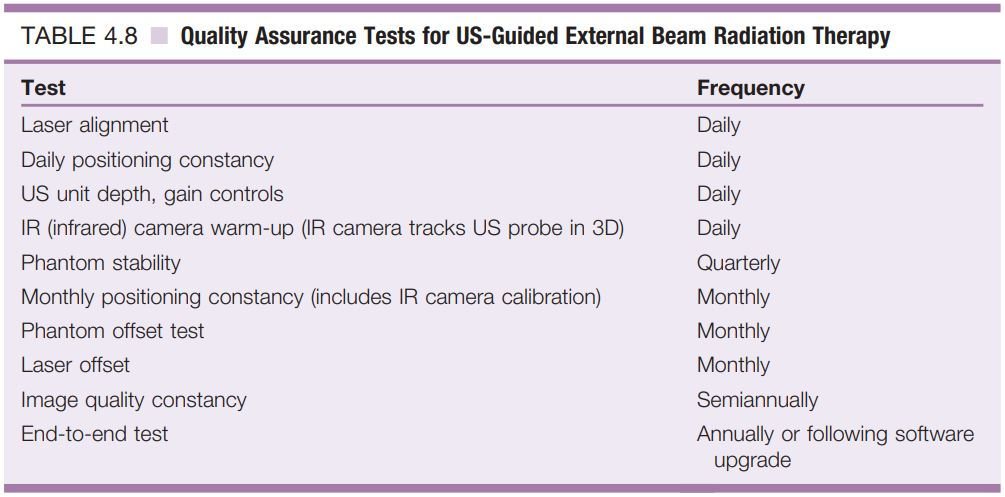
\includegraphics[width=0.7\textwidth]{Imagens/qaustele.JPG}
		}%
		\caption{Testes para US em teleterapia}
		\label{fig:qaustele}
	\end{figure}

	\begin{figure}[!h]
		\centering
		\fcolorbox{DarkTurquoise}{white}{%
			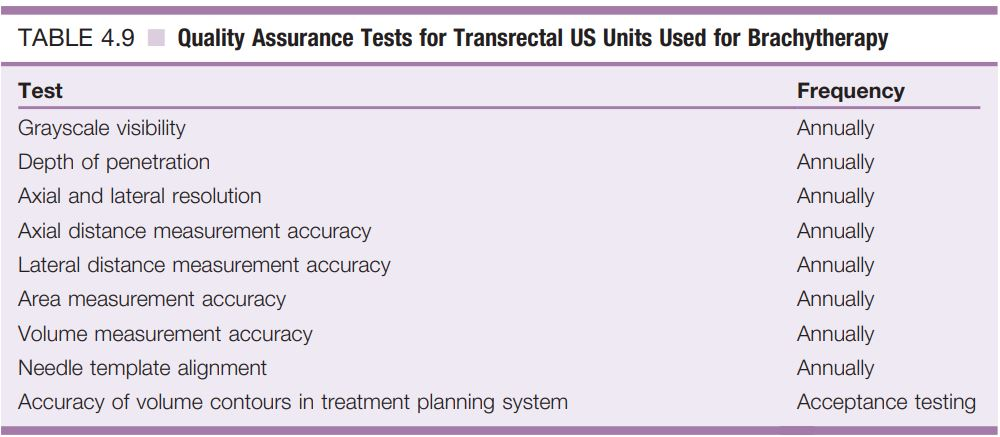
\includegraphics[width=0.7\textwidth]{Imagens/qausbraq.JPG}
		}%
		\caption{Testes para US em braquiterapia}
		\label{fig:qausbraq}
	\end{figure}

	Ambos requerem o uso de um phantom, que pode ser incluído no sistema ou adquirido separadamente. Estes phantoms são geralmente baseados em gel que têm uma vida útil limitada de modo que precisam ser substituídos periodicamente. Uma questão específica da \textcolor{MediumOrchid}{\textbf{\textit{US de braquiterapia de próstata}}} é o \textcolor{MediumOrchid}{\textbf{\textit{uso de um afastamento (standoff) em torno da sonda de US transretal}}}. Foi demonstrado que eles podem causar \textcolor{MediumOrchid}{\textbf{\textit{distorção de imagem}}} levando a determinação imprecisa do volume, posicionamento da agulha e cálculo da dose. O afastamento deve ser cuidadosamente testado antes do uso.

\subsection*{Unidades de PET e PET/CT}

	As unidades de tomografia por emissão de pósitrons (PET)/CT também estão se tornando mais comuns nos departamentos de Oncologia de Radiação. \textcolor{MediumOrchid}{\textbf{\textit{O controle de qualidade do componente PET pode estar fora da especialidade do físico médico da Radioterapia}}}, e um físico da medicina nuclear qualificado deve ser consultado. A Agência Internacional de Energia Atômica (IAEA) publicou um documento sobre QA para sistemas PET e PET/CT. O documento da IAEA é muito detalhado e inclui uma visão geral da tecnologia, bem como testes de aceite e descrições de controle de qualidade de rotina. \textcolor{MediumOrchid}{\textbf{\textit{O uso quantitativo de imagens PET depende do cálculo do valor de captação padronizado (SUV)}}}. O SUV é a \textcolor{MediumOrchid}{\textbf{\textit{razão entre a concentração de radioatividade derivada da imagem e a radioatividade injetada dividida pelo peso corporal do paciente}}}. Isso é feito para eliminar diferenças de valores devido a diferentes atividades injetadas e diferentes massas corporais. Como o SUV é importante na determinação de áreas malignas e seu delineamento preciso, a consistência do SUV deve ser verificada.

\subsection*{Unidades de Ressonância Magnética}

	Unidades de ressonância magnética (RM) dedicadas à Radioterapia estão se tornando cada vez mais comuns, embora ainda em minoria. Além disso, agora existem unidades de tratamento com capacidade de aquisição de imagem de RM. Como a física da RM geralmente está fora da especialidade de um físico médico em radioterapia, o controle de qualidade do sistema deve ser coordenado com um físico de RM qualificado. As recomendações do \textcolor{MediumOrchid}{\textbf{\textit{Relatório 100 da AAPM}}},  \textit{``Acceptance Testing and Quality Assurance Procedures for Magnetic Resonance Imaging Facilities''}, devem ser seguidas. O teste inclui \textcolor{MediumOrchid}{\textbf{\textit{medições de vibração}}}, \textcolor{MediumOrchid}{\textbf{\textit{teste de blindagem de RF}}}, \textcolor{MediumOrchid}{\textbf{\textit{mapeamento de campo de franja magnética}}}, \textcolor{MediumOrchid}{\textbf{\textit{testes de sistema mecânico}}}, \textcolor{MediumOrchid}{\textbf{\textit{testes de sistema de emergência}}}, \textcolor{MediumOrchid}{\textbf{\textit{testes de equipamentos de monitoramento de pacientes}}}, \textcolor{MediumOrchid}{\textbf{\textit{testes de subsistema de campo magnético estático}}}, \textcolor{MediumOrchid}{\textbf{\textit{testes de subsistema de RF}}}, \textcolor{MediumOrchid}{\textbf{\textit{testes de subsistema de gradiente}}}, \textcolor{MediumOrchid}{\textbf{\textit{testes combinados de sistema de gradiente/RF}}}, \textcolor{MediumOrchid}{\textbf{\textit{testes de imagem ultra-rápidos}}} e \textcolor{MediumOrchid}{\textbf{\textit{testes de espectroscopia}}}. O departamento deve estar ciente das sequências de pulso usadas para obter diferentes informações e delineamento ideal do alvo.

	Uma preocupação particular para unidades de tratamento com imagens de RM é a \textcolor{MediumOrchid}{\textbf{\textit{funcionalidade do equipamento de QA em um ambiente de alto campo magnético}}}. Não apenas o \textcolor{MediumOrchid}{\textbf{\textit{equipamento deve ser não ferroso}}}, mas a \textcolor{MediumOrchid}{\textbf{\textit{eletrônica também deve operar nesse ambiente}}}. Outros \textcolor{MediumOrchid}{\textbf{\textit{equipamentos que devem ser conectados à alimentação AC}}} ou \textcolor{MediumOrchid}{\textbf{\textit{usar cabos}}} para conectar dispositivos na sala de tratamento a dispositivos na sala de controle (ou seja, câmara de ionização ao eletrômetro) podem criar um \textcolor{MediumOrchid}{\textbf{\textit{efeito de antena}}} e distorcer as imagens de RM. Uma solução é colocar um eletrômetro operado por bateria dentro da sala de tratamento e obter as leituras usando a câmera de monitoramento. Dispositivos QA podem ser verificados quanto a conteúdo ferroso usando um ímã de mão.

	Se forem usados dispositivos de imobilização ou uma mesa plana, eles também devem ser verificados quanto à compatibilidade com RM. A \textcolor{MediumOrchid}{\textbf{\textit{fibra de carbono}}}, por exemplo, \textcolor{MediumOrchid}{\textbf{\textit{pode aquecer em campos magnéticos fortes devido à criação de correntes de Foucault}}}. Por causa disso, as encaixes de mesa plana e outros dispositivos são geralmente feitos de \textcolor{MediumOrchid}{\textbf{\textit{fibra de vidro}}}, que não apresenta essa propriedade.

	Finalmente, a segurança da equipe e do paciente é um fator importante no ambiente de RM. A área deve ser projetada para controlar e limitar o acesso, e sinalização clara deve estar presente. A equipe que entra nas áreas de campo elevado deve receber treinamento especializado regular sobre segurança em RM.

\section{Equipamentos Auxiliares}

	Além dos complexos equipamentos de geração de imagem e tratamento, existem muitos dispositivos auxiliares em um departamento de Radioterapia que exigem controle de qualidade. A \ref{fig:dispAux} lista alguns exemplos desses dispositivos e como eles podem ser testados.

	\begin{figure}[!h]
		\centering
		\fcolorbox{DarkTurquoise}{white}{%
			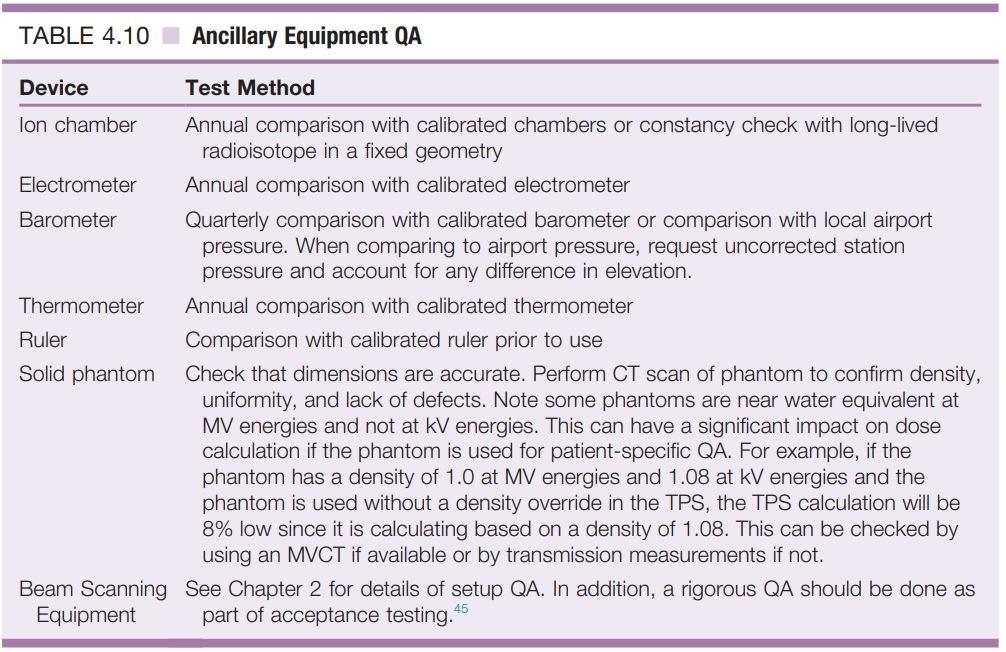
\includegraphics[width=0.7\textwidth]{Imagens/dispAux.JPG}
		}%
		\caption{QA de dispositivos auxiliares}
		\label{fig:dispAux}
	\end{figure}

\section{QA da Transferência de Dados}

	Dados em muitas formas são transferidos entre muitos sistemas em um departamento de Radioterapia. Um método sistemático é necessário para validar a precisão dos dados transferidos em cada etapa. Isso pode ser feito por \textcolor{MediumOrchid}{\textbf{\textit{inspeção visual de valores de parâmetros, revisão qualitativa das imagens ou através de métodos de comparação com arquivos mais elaborados}}}. O TG-201 descreve esses processos em grande detalhe.

\section{Avaliação do Programa de Garantia da Qualidade}

	Estabelecer e manter um programa abrangente de controle de qualidade em Radioterapia é um processo complexo e demorado. A quantidade de dados acumulada ao longo de um ano pode chegar a milhares de resultados discretos. Muitos dos dados serão simplesmente de natureza ``aprovada/reprovada'' e os resultados são simplesmente interpretados. Reports regulares desses dados devem ser feitos em reuniões mensais de controle de qualidade. Outros dados devem ser analisados em uma escala mais global. Por exemplo, foram feitas mudanças na política clínica que exigiriam a adoção de tolerâncias mais rígidas para alguns testes de controle de qualidade? Os resultados do QA de imagem são consistentes com as margens PTV usadas clinicamente? As políticas e procedimentos também devem ser revisados regularmente para confirmar se atendem aos regulamentos e recomendações mais recentes.

	Esses tipos de revisões podem estabelecer se os testes atuais estão ou não dentro dos limites atuais, mas não abordam nenhuma deficiência do programa. Revisões internas podem ser feitas para resolver isso, mas é melhor ter \textcolor{MediumOrchid}{\textbf{\textit{auditorias independentes}}}. O credenciamento da prática é uma maneira de conseguir isso. De fato, o credenciamento pode se tornar obrigatório em um futuro próximo. 

	Um estado dos Estados Unidos (NY) já o tornou obrigatório. Nos Estados Unidos, o credenciamento da prática pode ser realizado por meio do ACR ou, a partir de 2015, por meio do Programa de Credenciamento para Excelência (APEx) da ASTRO. O recredenciamento geralmente ocorre em um ciclo de 3 a 4 anos, portanto, há uma dúvida quanto aos requisitos nos anos intermediários. Esta é uma área provável para auditorias internas, embora as auditorias externas sejam preferidas porque uma opinião externa tem muito mais probabilidade de identificar áreas para melhoria. Isso pode ser feito por meio de um acordo informal com um colega ou um contrato formal com um físico consultor. O \textcolor{MediumOrchid}{\textbf{\textit{TG-103}}}, ``Peer Review in Clinical Radiation Oncology Physics'', descreve os componentes e expectativas de uma revisão externa.

	Auditorias de dosimetria de rotina também são recomendadas e geralmente necessárias para a participação em ensaios clínicos. Fora de qualquer auditoria de dosimetria necessária, todo feixe de tratamento deve receber verificação externa da dose absoluta anualmente (no Brasil é a cada 2 anos segundo a norma 6.10 da CNEN). Os serviços de dosimetria estão disponíveis no IROC (anteriormente RPC), University of Wisconsin e IAEA. Além disso, é uma boa prática realizar anualmente auditorias multidimensionais modalidade-específica para as técnicas oferecidas na clínica. Por exemplo, se uma instalação oferece IMRT, SRS e SBRT, uma auditoria de dosimetria pode ser feita anualmente de forma rotativa: IMRT no ano 1, SRS no ano 2 e SBRT no ano 3, por exemplo.

	A CNEN participou de uma discussão com a ABFM para estabelecer os requisitos mínimos de um programa de auditoria externa. A CNEN ainda está aceitando o programa do PQRT do inca como auditoria externa, porém em breve não será mais aceito. 

	Os requisitos mínimos de uma Auditoria Externa foram divididos em tópicos sendo Aceleradores Lineares, Braquiterapia e TPS, onde para cada um desses tópicos estão definidos os parâmetros que precisam ser verificados e os parâmetros que precisam ser medidos incluindo a verificação E2E. Também foi incluída a avaliação dos equipamentos de dosimetria.

\subsubsection*{Teste End-To-End}

	O primeiro passo é realizar uma tomografia de um fantoma homogêneo que será utilizado para as medidas. Caso o serviço não possua tomografia ou não seja dedicado, uma alternativa é apenas importar as imagens deste phantom nos sistemas de planejamento, o que é uma opção aceitável, mas não a ideal. 
	
	Após a aquisição das imagens, a segunda etapa consiste no planejamento, iniciando co  a importação das imagens e verificando como essas imagens são transferidas para o sistema de planejamento. Nesta etapa, serão criados planos de teste para verificar o cálculo (por energia disponível), como campos individuais diretos com e sem filtro (se aplicável), um plano 3D que representa a rotina de tratamento (com no mínimo 3 campos). Caso o setor possua máquinas com elétrons, recomenda-se que os planos sejam calculados com pelo menos uma energia e um cone, em duas SSDs diferentes. Os planos devem ser tratados como um paciente,ou seja, agendados no sistema de gerenciamento, aprovados e utilizados para verificação do sistema	de cálculo da unidade independente de monitoramento (UM) (mesmo que seja manual). Ao realizar todos esses procedimentos, vários parâmetros importantes já estarão medidos, como a transferência de dados e cálculo de UM.

	A terceira etapa é a execução desses planos nos equipamentos de tratamento como se fosse um tratamento padrão, ou seja, utilizando o sistema de gerenciamento. Esses planos devem ser executados usando o mesmo fantoma e um sistema de verificação de dose independente do equipamento de tratamento. Ao realizar esta etapa, é possível verificar a transferência de dados do sistema de planejamento para o equipamento de tratamento, sistema de registro do tratamento, dose medida em um ponto e/ou distribuição planar de dose. 

	A quarta etapa consiste em comparar os parâmetros medidos com os calculados. Desta forma, é possível verificar o cálculo de dose de um campo aberto, a distribuição de dose, os fatores fora do eixo, fatores de filtro, fatores de cone.


\subsubsection*{Aceleradores Lineares}

	A \ref{fig:aeAlVerif}, \ref{fig:aeAlMed} e \ref{fig:aeAle2e} mostra os parâmetros definidos para serem avaliados na Auditoria Externa de Aceleradores Lineares.

	\begin{figure}[h]
		\centering
		\fcolorbox{DarkTurquoise}{white}{%
			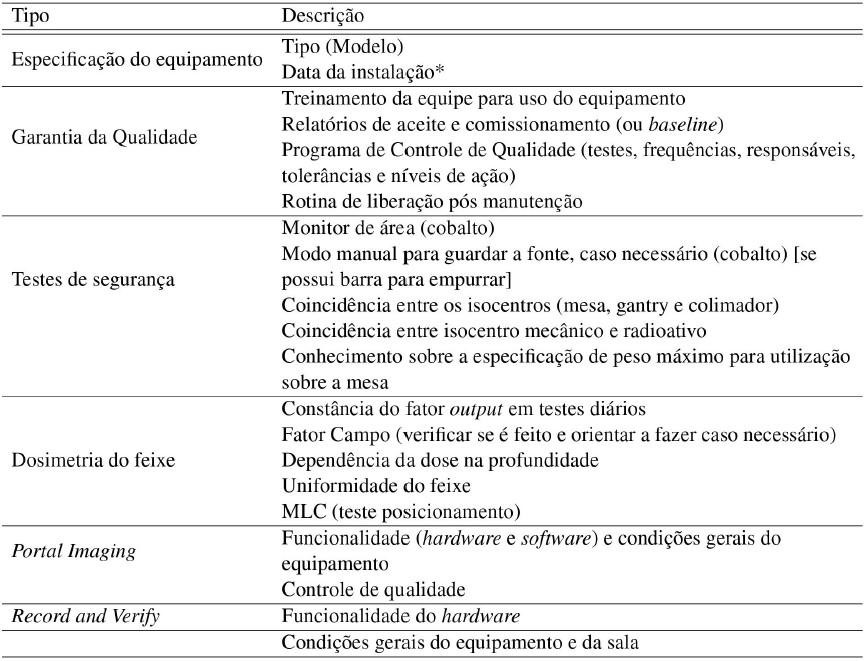
\includegraphics[width=0.5\textwidth]{Imagens/aeAlVerif.jpg}
		}%
		\caption{Itens a serem verificados em aceleradores lineares durante auditoria externa.}
		\label{fig:aeAlVerif}
	\end{figure}

	\begin{figure}[h]
		\centering
		\fcolorbox{DarkTurquoise}{white}{%
			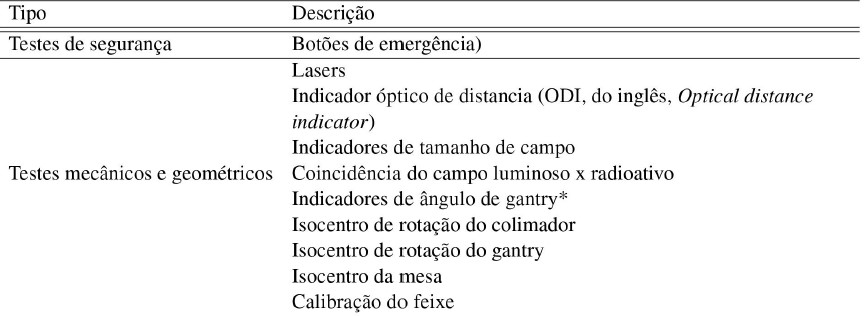
\includegraphics[width=0.5\textwidth]{Imagens/aeAlMed.jpg}
		}%
		\caption{Itens a serem medidos ou avaliados em aceleradores lineares durante auditoria externa.}
		\label{fig:aeAlMed}
	\end{figure}

	\begin{figure}[h]
		\centering
		\fcolorbox{DarkTurquoise}{white}{%
			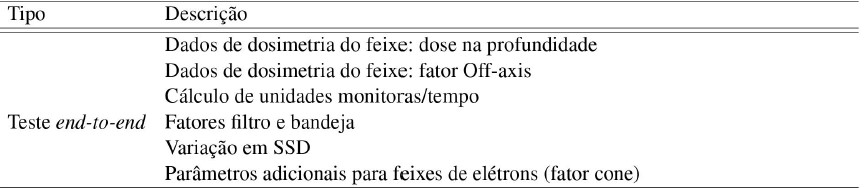
\includegraphics[width=0.5\textwidth]{Imagens/aeAle2e.jpg}
		}%
		\caption{Itens a serem medidos ou avaliados através de testes end-to-end em aceleradores lineares durante auditoria externa.}
		\label{fig:aeAle2e}
	\end{figure}

\subsubsection*{Braquiterapia}

	A \ref{fig:aeBqVeri} e \ref{fig:aeBqe2e} mostra os parâmetros definidos para serem avaliados na Auditoria Externa dos Sistemas de Braquiterapia.

	\begin{figure}[h]
		\centering
		\fcolorbox{DarkTurquoise}{white}{%
			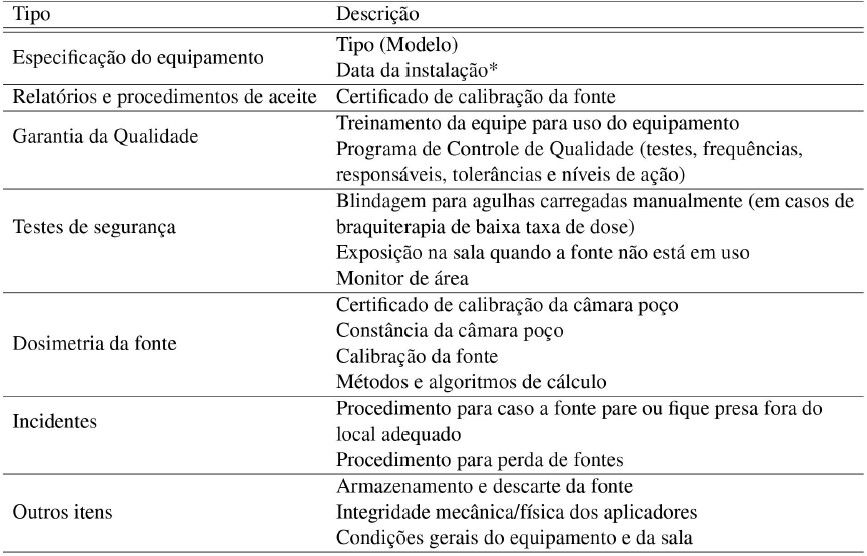
\includegraphics[width=0.5\textwidth]{Imagens/aeBqVeri.jpg}
		}%
		\caption{Itens a serem verificados na braquiterapia durante auditoria externa.}
		\label{fig:aeBqVeri}
	\end{figure}

	\begin{figure}[h]
		\centering
		\fcolorbox{DarkTurquoise}{white}{%
			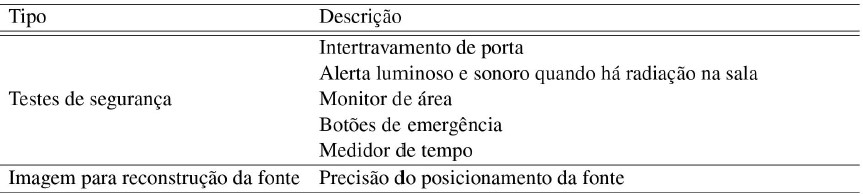
\includegraphics[width=0.5\textwidth]{Imagens/aeBqe2e.jpg}
		}%
		\caption{Itens a serem medidos ou avaliados na braquiterapia durante auditoria externa.}
		\label{fig:aeBqe2e}
	\end{figure}

\subsubsection*{TPS}

	A \ref{fig:aeTpsBraqVeri} e \ref{fig:aeTpsTeleE2e} mostra os parâmetros definidos para serem avaliados na Auditoria Externa do TPS.

	\begin{figure}[h]
		\centering
		\fcolorbox{DarkTurquoise}{white}{%
			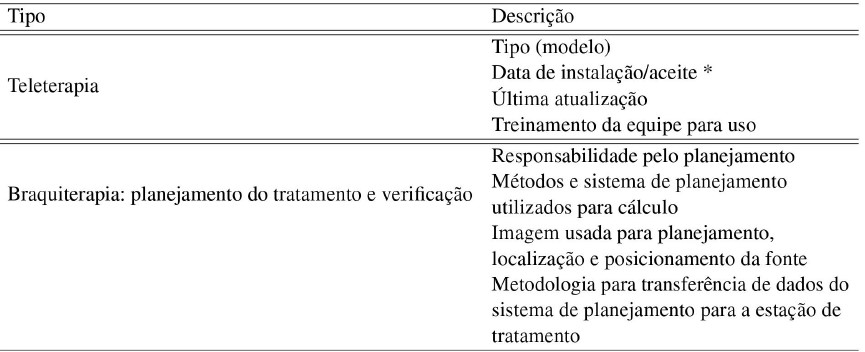
\includegraphics[width=0.5\textwidth]{Imagens/aeTpsBraqVeri.jpg}
		}%
		\caption{Itens a serem verificados no TPS de Braquiterapia e Teleterapia durante auditoria externa.}
		\label{fig:aeTpsBraqVeri}
	\end{figure}

	\begin{figure}[h]
		\centering
		\fcolorbox{DarkTurquoise}{white}{%
			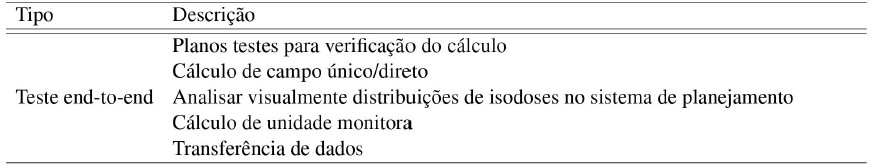
\includegraphics[width=0.5\textwidth]{Imagens/aeTpsTeleE2e.jpg}
		}%
		\caption{Itens a serem medidos ou avaliados através de testes end-to-end no TPS durante auditoria externa.}
		\label{fig:aeTpsTeleE2e}
	\end{figure}

\subsubsection*{Cálculo de Dose}

	A \ref{fig:aeTpsDose} mostra os parâmetros definidos para serem avaliados na Auditoria Externa quanto à determinação da dose.

	\begin{figure}[h]
		\centering
		\fcolorbox{DarkTurquoise}{white}{%
			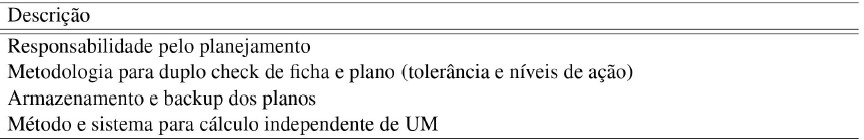
\includegraphics[width=0.5\textwidth]{Imagens/aeTpsDose.jpg}
		}%
		\caption{Itens a serem verificados quanto ao cálculo da dose durante auditoria externa.}
		\label{fig:aeTpsDose}
	\end{figure}


\section{Direções Futuras no Controle de Qualidade}

	O teste de aceite, o comissionamento e o controle de qualidade contínuo do equipamento de radioterapia são vitais para a entrega precisa da radiação. Existem muitas referências que descrevem as considerações técnicas dessas atividades. Igualmente importante é ter um processo abrangente de testes, identificação de riscos, treinamento de toda a equipe envolvida, documentação de políticas e procedimentos, desenvolvimento do processo de controle de qualidade e desenvolvimento de métricas de desempenho. Os documentos de referência e as informações do fornecedor, juntamente com a avaliação de risco, orientarão os testes. Os riscos podem ser identificados usando processos como modo de falha e análise de efeito (FMEA - a sigla em inglês failure mode and effect analysis) ou através do Sistema de Avaliação de Risco em Radioterapia (SEVRRA – da sigla em espanhol para Sistema de Evaluación del Riesgo en Radioterapia). O treinamento será orientado pelo fornecedor e as informações serão obtidas durante o processo de teste. Para implementar uma nova tecnologia com segurança, todos os funcionários devem ter uma compreensão clara de suas funções, que são bem descritas pelas políticas e procedimentos. A precisão e a segurança contínuas do sistema devem ser monitoradas por um programa abrangente de controle de qualidade. Existem muitas referências técnicas que descrevem programas de QA para a maioria dos sistemas, mas também há um movimento crescente para projetar programas de QA com base em avaliações de risco. Uma vez que o sistema esteja em uso clínico, métricas devem ser desenvolvidas para monitorar a eficácia clínica. Por exemplo, se um programa de SBRT for implementado, os resultados clínicos devem ser verificados após o primeiro grupo de pacientes para garantir que os objetivos do programa tenham sido alcançados e que não haja efeitos agudos inesperados. Dois temas comuns percorrem esses processos: identificar e gerenciar riscos e garantir a competência da equipe.


\bibliography{ref.bib}
\end{document}